\PassOptionsToPackage{authoryear,round}{natbib}
\documentclass[11pt,twocolumn]{article}
\usepackage{report}

\usepackage{hyperref}       % hyperlinks
\usepackage{url}            % simple URL typesetting
\usepackage{booktabs}       % professional-quality tables
\usepackage{amsfonts}       % blackboard math symbols
\usepackage{nicefrac}       % compact symbols for 1/2, etc.
\usepackage{microtype}      % microtypography
\usepackage{graphicx}
\usepackage{amsmath}
\usepackage{titling}
\usepackage{caption}
\usepackage{subcaption}
\captionsetup{labelsep=period}
%\usepackage[font=small]{caption}
\setlength{\droptitle}{-40pt}  % Adjust as needed


\usepackage{amssymb}
\usepackage{pifont}
\newcommand{\cmark}{\checkmark}
\newcommand{\xmark}{\ding{55}}

\usepackage{titlesec}

\titlespacing{\section}
  {0pt}    % left margin
  {0.7ex plus 0.5ex minus .2ex}  % space before section title
  {0.7ex plus .2ex}  % space after section title (before paragraph)

\titlespacing{\subsection}
  {0pt}
  {1.2ex plus 0.3ex minus .2ex}
  {0.6ex plus .1ex}

\title{\vspace{-1em}{\Large\textbf{Garment Texture Completion in UV space using Diffusion}}\vspace{-1em}}

\author{
  \begin{tabular}{c c}
  Ludek Cizinsky & Yingxuan You\thanks{Yingxuan provided the initial idea, and model pipeline based on her previous work. She then provided Ludek with the helpful feedback throughout the semester.}  \\
  \texttt{ludek.cizinsky@epfl.ch} & \texttt{yingxuan.you@epfl.ch} \\
  EPFL & EPFL
  \end{tabular}
}

\begin{document}

\date{}
\maketitle

\section{Introduction}\label{sec:intro}

There is an increasing interest in digitalising garments, that is, converting an image of a person wearing clothing into a 3D model of the depicted garments. In this work, we focus specifically on extracting high-quality physically based rendering (PBR) texture maps, while relying on a pre-trained Human Vision Model to handle the geometry. PBR texture maps are essential for realistic rendering of garment appearance and are thus of particular importance for downstream applications in gaming and the film industry. However, most existing methods extract only RGB texture maps, which include baked-in lighting from the original environment, limiting their adaptability and usefulness for other scenes or renderers.

Extracting high-quality PBR texture maps from a single RGB image poses several challenges. First, the problem involves modeling both the geometry and the appearance of the garment. Input images typically vary in lighting conditions and camera positions, making it difficult to disentangle material properties from illumination. In addition, garments themselves introduce domain-specific complications: self-occlusions often obscure parts of the fabric, which hinders accurate pattern capture; logos may be difficult to isolate and are frequently overlaid on the fabric in ways that complicate extraction; and finally, garment textures exhibit significant variation, ranging from simple, repetitive motifs to complex, irregular patterns.

Most prior work has concentrated on the geometry, while texture modeling is usually simplified to generating RGB texture maps, as seen in methods such as \textit{Garment3DGen} \cite{garment3dgen}, \textit{DeepIron} \cite{deepiron}, or \textit{Wordrobe} \cite{WordRobe}. To the best of our knowledge, \textit{Fabric Diffusion} (FBD) \cite{fabricdiffusion} is the only method that directly attempts to generate PBR texture maps from a single image. However, this approach comes with limitations. FBD relies on a user-provided patch of the garment to model local texture patterns, assuming these can be seamlessly tiled to cover the surface. This assumption fails when patterns are not globally repetitive, and it may produce unnatural seams between tiles. Additionally, logo extraction in FBD requires the user to manually crop the logo, after which the model removes background and lighting artifacts. While effective in isolated cases, this process is impractical for full-garment digitalisation and does not generalise well to garments with multiple logos.

A further bottleneck in this field is the absence of a large-scale public dataset that pairs garment images with corresponding PBR texture maps. This data gap presents a key obstacle to training more robust and generalisable models for PBR texture extraction from images.

In this paper, we take a first step toward scalable, fully-automated garment digitalization by addressing the task of UV-space texture inpainting. Given a partially observed diffuse texture map, our goal is to complete the garment appearance in UV space. For simplicity, we do not address logo modeling in this work.

To inform our method design, we conduct a systematic evaluation of key training and inference choices. We ask: (1) What are the optimal text and image guidance scales during inference? (2) What is the best initialization strategy for fine-tuning? (3) How do training set size and duration affect model performance?

We find that a text guidance scale of 1.5 and image scale of 5.0 yield the best results. Further, initializing from InstructPix2Pix and fine-tuning only LoRA weights leads to superior performance. Surprisingly, we observe that training on only 5k images performs nearly as well as using the full 27k set, although longer training time consistently improves results.

\section{Related Work}

\textbf{General Material Texture Generation.} \textit{TexGen}~\cite{texgen} proposes a generative model for RGB texture synthesis in UV space, 
conditioned on either image or text inputs, and integrates 3D geometry information into the texture generation pipeline. 
\textit{Material Palette}~\cite{materialpalette} targets PBR material extraction from single images of 
real-world surfaces and introduces LoRA-based fine-tuning of diffusion models. 
\textit{DreamPBR}~\cite{dreampbr} and \textit{DreamMat}~\cite{dreammat} explore high-quality PBR texture generation from text, with the 
former supporting multi-modal inputs including fabric-related prompts. 
However, their models are either unpublished or lack garment-specific outputs such as normal maps. 
\textit{MatFusion}~\cite{matfusion} addresses the removal of baked-in lighting from input images for SVBRDF 
estimation and serves as a key component in \textit{FabricDiffusion}'s PBR extraction pipeline. Our work draws 
inspiration from these advances while focusing specifically on recovering garment-specific PBR maps from a single image.

\textbf{Garment Texture Generation.} \textit{FabricDiffusion}~\cite{fabricdiffusion} proposes a two-stage pipeline that first normalizes RGB garment textures 
and then employs an external model to predict the corresponding PBR texture maps, leveraging prior SVBRDF estimation techniques. 
\textit{Garment3DGen}~\cite{garment3dgen} introduces a multi-stage framework for 3D garment modeling, combining geometry and texture streams into a 
renderable output; however, it relies solely on RGB textures. Similarly, \textit{DeepIron}~\cite{deepiron} presents a pipeline involving garment segmentation, 
texture unwrapping, and inpainting, followed by application of the recovered texture onto a predefined sewing pattern, 
with its main novelty being the learned unwarping module. Our approach differs in focusing explicitly on recovering garment-specific PBR maps for the 
entire garment (not just a patch like in \textit{FabricDiffusion}) enabling higher realism and better generalization across lighting conditions.

\textbf{3D Garment Generation.}  
\textit{DressCode}~\cite{dresscode} introduces a multi-stage framework for text-driven garment synthesis, combining an autoregressive model that generates sewing patterns from prompts with a conditional diffusion model that produces corresponding PBR textures. \textit{WordRobe}~\cite{WordRobe} maps text inputs to textured 3D garments via a disentangled latent garment space and CLIP-based alignment, but produces only RGB textures. \textit{Design2Cloth}~\cite{design2cloth} enables mask-guided 3D garment generation and releases a large dataset of over 2{,}000 real-world garment scans. \textit{PICTURE}~\cite{picture} offers greater design flexibility by disentangling garment style and texture, employing a two-stage pipeline that first predicts garment shape and then generates texture conditioned on that shape. Finally, \textit{VTON360}~\cite{vton360} addresses the challenge of viewpoint consistency in virtual try-on, introducing a method for generating high-fidelity garments renderable from arbitrary angles.  
All these approaches focus on end-to-end 3D garment generation. In contrast, our method focuses specifically on high-quality \textit{texture reconstruction} from real images, aiming to recover physically meaningful material properties. As such, it can serve as a plug-in module for enhancing the realism and generalizability of generative pipelines that rely on RGB textures or simplified appearance models.


\section{Method}

\begin{figure*}[!t]
  \centering
  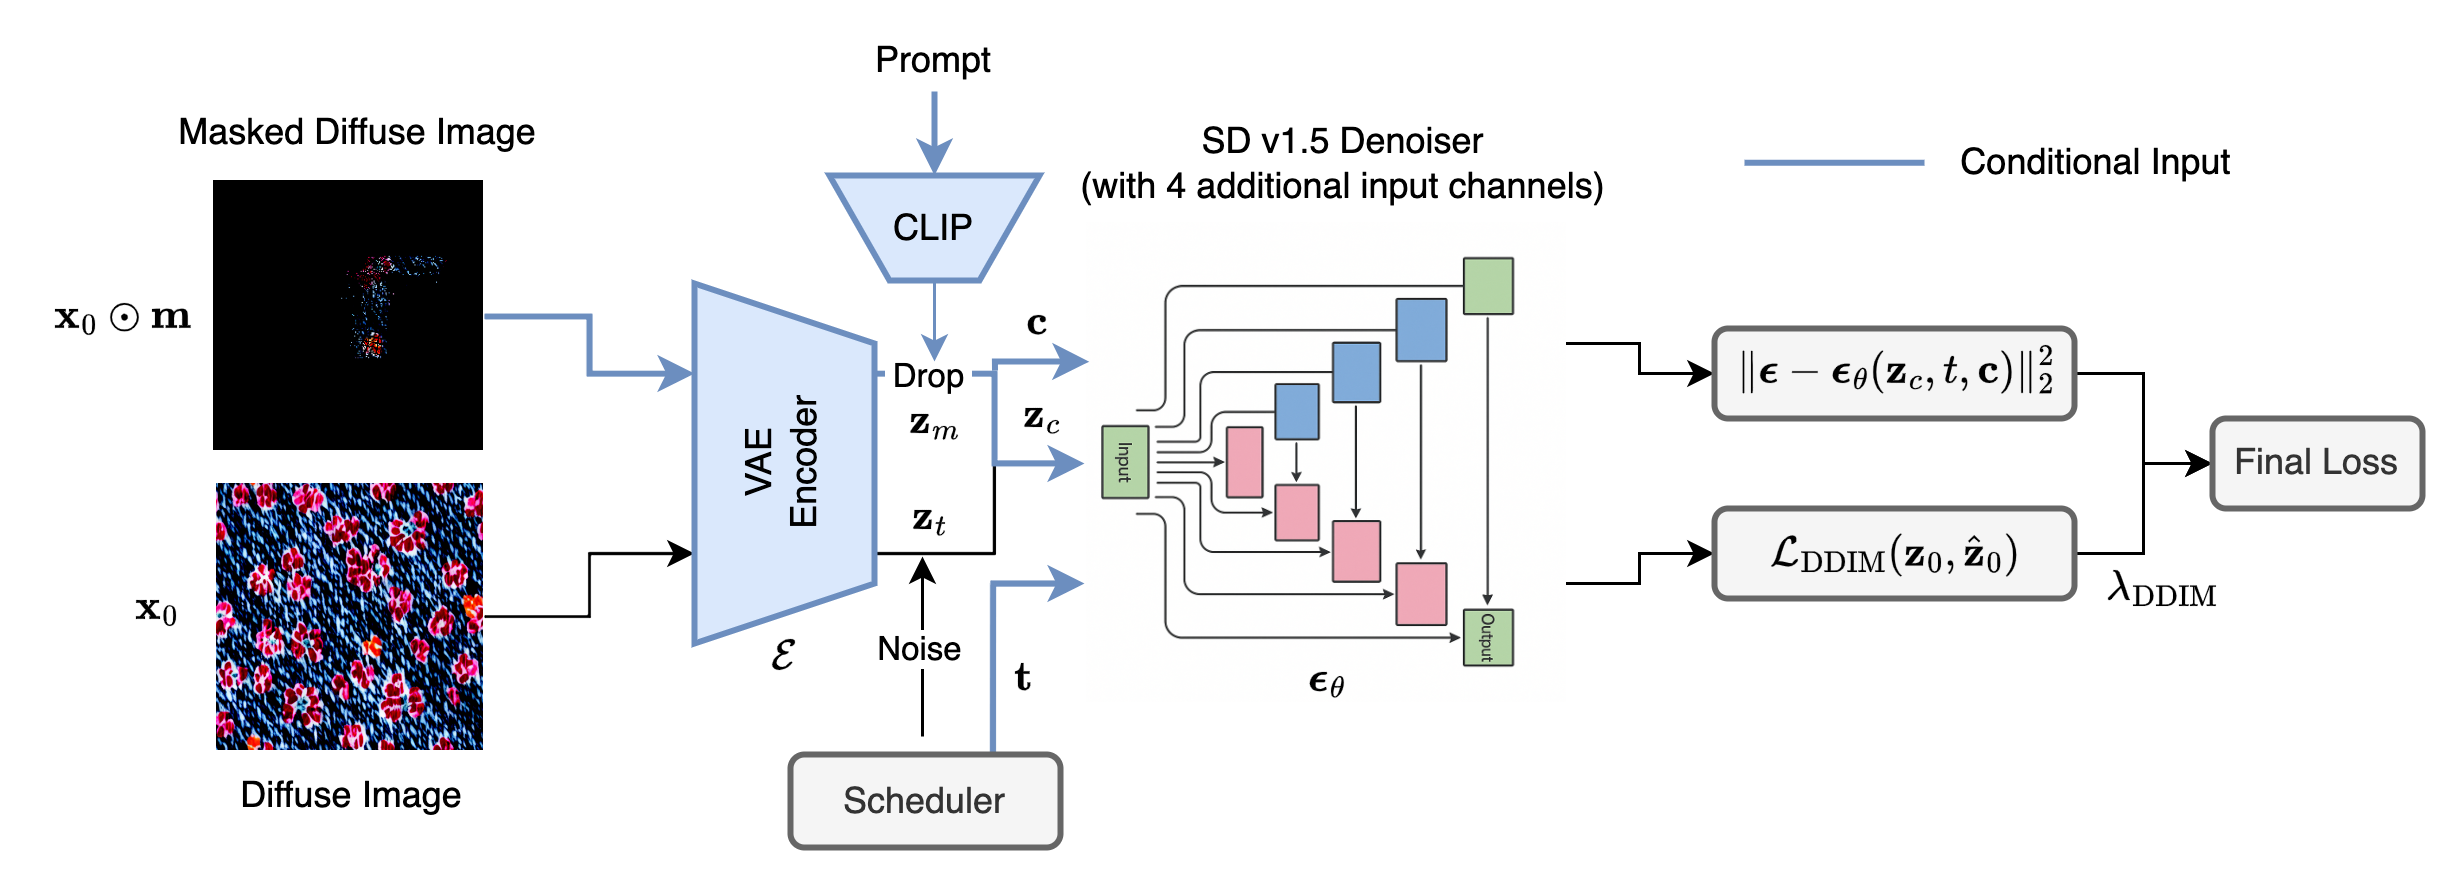
\includegraphics[width=0.8\textwidth]{figures/pbr_train_overview.png}
  \caption{Overview of the training pipeline.}
  \label{fig:trn-overview}
\end{figure*}

We make use of a pre-trained VAE \cite{vae} encoder-decoder pair $(\mathcal{E}, \mathcal{D})$ for diffuse textures, where $\mathcal{E}: \mathbb{R}^{H \times W \times 3} \rightarrow \mathbb{R}^{C \times H' \times W'}$ encodes RGB images into a latent space, and $\mathcal{D}$ maps latents back to image space. The decoder was specifically fine-tuned for the task of reconstructing diffuse textures \cite{dresscode}.

Figure \ref{fig:trn-overview} shows an overview of our fine tuning pipeline. Given an input diffuse texture $\mathbf{x}_0$ and a binary mask $\mathbf{m}$, we encode the full and masked textures using the VAE encoder:
$$
\mathbf{z}_0 = \mathcal{E}(\mathbf{x}_0), \quad \mathbf{z}_m = \mathcal{E}(\mathbf{x}_0 \odot \mathbf{m}),
$$

where $\odot$ denotes element-wise multiplication. We then sample a timestep $t \sim \mathcal{U}(1, T)$, using PNDM scheduler \cite{pndm}, and generate a noisy latent:
\vspace{0.0em}
$$
\mathbf{z}_t = \sqrt{\bar{\alpha}_t} \mathbf{z}_0 + \sqrt{1 - \bar{\alpha}_t} \boldsymbol{\epsilon}, \quad \boldsymbol{\epsilon} \sim \mathcal{N}(0, \mathbf{I}),
$$

where $\bar{\alpha}_t$ is the cumulative product of noise schedule coefficients. A conditioning text prompt $\mathbf{c}$ (constant across all samples) is embedded using CLIP \cite{clip}. To enable classifier-free guidance \cite{cfg}, we randomly drop the conditioning with some probability $p_{\text{drop}}$.

The model $\boldsymbol{\epsilon}_\theta$ is trained to predict the noise $\boldsymbol{\epsilon}$ added to $\mathbf{z}_0$. The total loss is then a weighted sum of the denoising objective and a DDIM reconstruction loss:
$$
\mathcal{L} = \|\boldsymbol{\epsilon} - \boldsymbol{\epsilon}_\theta(\mathbf{z}_t, t, \mathbf{c})\|_2^2 + \lambda_{\text{DDIM}} \cdot \mathcal{L}_{\text{DDIM}}(\mathbf{z}_0, \hat{\mathbf{z}}_0),
$$

where $\hat{\mathbf{z}}_0$ is the model's reconstruction using DDIM inversion \cite{ddim} and $\lambda_{\text{DDIM}}$ is the weight of DDIM loss.

During inference, we adopt the same approach as in \textit{InstructPix2Pix} \cite{instructpix2pix}, 
where we condition the diffusion model on latents of the masked texture $\mathbf{z}_m$ and text prompt 
$\mathbf{z_c}$ to iteratively denoise from the noisy input image $\mathbf{z}_T$ to $\hat{\mathbf{z}}_0$. 
Importantly, we make use of classifier-free guidance \cite{cfg} to enable control over the text prompt and 
image guidance influence on the final texture. Based on our experiments, we find the text guidance scale $w_T = 1.5$ 
and image guidance scale $w_I = 5.0$ to be optimal.
\vspace{0.0em}
\begin{align*}
  \tilde{\boldsymbol{\epsilon}}_{\theta}(\mathbf{z}_t, &\mathbf{c}_I, \mathbf{c}_T) = \boldsymbol{\epsilon}_{\theta}(\mathbf{z}_t, \varnothing, \varnothing) \\
  &\quad + w_I \cdot \left( \boldsymbol{\epsilon}_{\theta}(\mathbf{z}_t, \mathbf{c}_I, \varnothing) - \boldsymbol{\epsilon}_{\theta}(\mathbf{z}_t, \varnothing, \varnothing) \right) \\
  &\quad + w_T \cdot \left( \boldsymbol{\epsilon}_{\theta}(\mathbf{z}_t, \mathbf{c}_I, \mathbf{c}_T) - \boldsymbol{\epsilon}_{\theta}(\mathbf{z}_t, \mathbf{c}_I, \varnothing) \right)
\end{align*}

% SD v1.5 (img2img)
% SSIM: 0.02430877275764942, PSNR: 6.464392185211182, LPIPS: 0.9525905251502991

% SD v1.5 inpaint (inpatient)
% SSIM: 0.020838197320699692, PSNR: 6.564342498779297, LPIPS: 0.9757870435714722


\section{Results}

\begin{table*}[t] % top-aligned table
  \centering
  \begin{subtable}[t]{0.48\textwidth} % top alignment
    \vspace{0pt} % ensure top alignment
    \centering
    \begin{tabular}{l|ccc}
    \toprule
    \textbf{Model} & \textbf{LPIPS} $\downarrow$ & \textbf{SSIM} $\uparrow$ & \textbf{PSNR} $\uparrow$ \\
    \midrule
    Ours         & 0.45 & 0.17 & 13.04 \\
    SD-Inpaint & 0.97 & 0.02 & 6.56 \\
    Pix2Pix      & 1.00 & 0.03 & 6.36  \\
    SD  & 0.95 & 0.02 & 6.46 \\
    \bottomrule
    \end{tabular}
    \subcaption{Comparison to non-finetuned baselines.}
    \label{tab:best-vs-baseline}
  \end{subtable}
  \hfill
  \begin{subtable}[t]{0.48\textwidth} % top alignment
    \vspace{0pt} % ensure top alignment
    \centering
    \begin{tabular}{cc|ccc}
    \toprule
    \textbf{TNS} & \textbf{TT [hrs]} & \textbf{LPIPS} $\downarrow$ & \textbf{SSIM} $\uparrow$ & \textbf{PSNR} $\uparrow$ \\
    \midrule
    27,000 & 60 & 0.45 & 0.17 & 13.04 \\
    5,000 & 30 & 0.49 & 0.17 & 13.11 \\
    15,000 & 30 & 0.50 & 0.16 & 13.10 \\
    20,000 & 30 & 0.51 & 0.17 & 13.12 \\
    10,000 & 30 & 0.52 & 0.17 & 12.65 \\
    \bottomrule
    \end{tabular}
    \subcaption{Effect of training set size and time on performance.}
    \label{tab:scale-study}
  \end{subtable}
  \caption{Comparison of our best model against non-finetuned baselines and ablation study on effect of time and training set size scale.}
  \label{tab:base-and-scale}
\end{table*}


\begin{table*}[t]
  \centering

  \begin{subtable}[t]{\textwidth}
    \centering
    \vspace{0pt}
    \begin{tabular}{cccc|ccc}
    \toprule
    \textbf{DDIM Weight} & \textbf{LR} & \textbf{Cosine Scheduler LR} & \textbf{EMA} & \textbf{LPIPS} $\downarrow$ & \textbf{SSIM} $\uparrow$ & \textbf{PSNR} $\uparrow$ \\
    \midrule
    0.50 & 1e-04 & \xmark & \xmark & 0.45 & 0.17 & 13.04 \\
    0.75 & 1e-05 & \xmark & \xmark & 0.58 & 0.14 & 12.21 \\
    0.25 & 1e-05 & \xmark & \xmark & 0.63 & 0.12 & 12.08 \\
    0.50 & 1e-05 & \cmark & \xmark & 0.69 & 0.12 & 10.70 \\
    0.50 & 1e-05 & \xmark & \xmark & 0.69 & 0.09 & 9.88 \\
    0.50 & 1e-05 & \xmark & \cmark & 0.70 & 0.12 & 11.40 \\
    0.00 & 1e-05 & \xmark & \xmark & 0.78 & 0.06 & 10.07 \\
    0.50 & 3e-06 & \xmark & \xmark & 0.83 & 0.09 & 10.22 \\
    \bottomrule
    \end{tabular}
    \subcaption{Comparison of hyperparameter configurations and corresponding metrics.}
    \label{tab:hyperparams}
  \end{subtable}

  \vspace{1em} % spacing between the tables

  \begin{subtable}[t]{\textwidth}
    \centering
    \vspace{0pt}
    \begin{tabular}{ccccccc|ccc}
    \toprule
    \textbf{DDIM Weight} & \textbf{LR} & \textbf{BSZ} & \textbf{LoRA} & \textbf{Scratch} & \textbf{Inpaint} & \textbf{Base Model} & \textbf{LPIPS} $\downarrow$ & \textbf{SSIM} $\uparrow$ & \textbf{PSNR} $\uparrow$ \\
    \midrule
    0.50 & 1e-04 & 20 & \cmark & \xmark & \xmark & pix2pix & 0.61 & 0.12 & 12.15 \\
    0.50 & 1e-05 & 20 & \cmark & \xmark & \xmark & pix2pix & 0.76 & 0.10 & 10.62 \\
    0.50 & 1e-05 & 20 & \xmark & \cmark & \xmark & sd & 0.82 & 0.02 & 7.48 \\
    0.75 & 1e-04 & 10 & \xmark & \xmark & \cmark & sd-inpaint & 0.86 & 0.05 & 7.11 \\
    0.75 & 1e-04 & 20 & \cmark & \xmark & \cmark & sd-inpaint & 0.96 & 0.13 & 9.25 \\
    0.50 & 5e-03 & 40 & \cmark & \xmark & \xmark & pix2pix & - & - & - \\
    0.50 & 1e-04 & 40 & \cmark & \xmark & \xmark & pix2pix & - & - & - \\
    \bottomrule
    \end{tabular}
    \subcaption{Ablation study over model architecture and training strategy.}
    \label{tab:arch-ablation}
  \end{subtable}

  \caption{Effect of hyperparameters and architectural choices on model performance.}
  \label{tab:combined-hparams-arch}
\end{table*}




\newpage
\bibliographystyle{plainnat}
\bibliography{references}

\end{document}